%!TEX root = ../clcxsj.tex

\chapter{测量基础函数设计}

本章我们将编写一些测量程序设计中常用的函数,用于以后的测绘算法之中。

\section{C\# 知识点}

C\# 是纯面向对象语言,也就是说所有的常量与方法都需要以类$class$为载体。

C\#中的类分为实例类与静态类。实例类需要用关键字 new 将类实例化,在一些与类的实例成员操作无关的
环境中,对类进行实例化的操作显得冗余,而静态类与类的静态成员可以很好的解决这个问题。 

如果我们分析C\#系统中的System.Math类,我们会发现常用的一些数学函数都被设计成了静态函数。因此,我们也如同System.Math类一样,
也将我们常用的测绘算法也用类名$SMath(SurveyMath)$命名,保存在$SMath.cs$文件中,
将常用的一些常量及方法定义也定义为静态成员。

示例代码如下所示:
\begin{lstlisting}[language=C]
namespace ZXY
{
    public static class SMath
    {
        public const double PI=Math.PI;
        public const double TWOPI=2*Math.PI;
        public const double TODEG=180.0/PI; 
        public const double TORAD=PI/180.0;
        public const double TOSECOND=180.0*3600.0/PI;
    
        public static double DMStoRAD(double dmsAngle)
        {
            ......
        }
    
        public static double RADtoDMS(double radAngle)
        {
            ......
        }
    }
}
\end{lstlisting}

以上示例代码为了与其他的函数或符号相区别,也为了与其他的代码一起配合使用,
在此加入了自己的命名空间 ZXY (这是我用的名称空间,
你当然也可以根据自己的习惯或爱好命名适当的名称空间)。


\section{测绘常用算法设计}

\subsection{测绘算法中的常量}
角度、距离与高差是测量工程师工作的基本对象,度分秒形式的角度与弧度之间的转换是我们进行测量数据处理的基础。
为了方便的进行测量数据处理,我们首先需要定义一些常量,如上述示例代码所示,其中:

$PI$表示$\pi$, $TWOPI$表示$2\pi$;
$TODEG$表示$180/\pi$,用于将弧度化为度;
$TORAD$表示$\pi/180$,用于将度化为弧度;
$TOSECOND$表示$180*3600/\pi$,用于将弧度转换为秒。

在静态类SMath中我们采用常量const的形式定义了$\pi, 2\pi$等常用的数值,在 C\# 中 const类型的数据总是
静态的(static),而且是不需要static修饰符的。另外需注意,const类型的数据在声明时必须进行初始化,且其值
必须在编译时就能确定计算出。

\subsection{六十进制度分秒化弧度函数}

 在测量工程中角度的常用习惯表示法是度分秒的形式,
 在计算程序中测量工程人员也常将度分秒形式的角度用格式为xxx.xxxxx的形式表示,
 即以小数点前的整数部分表示度,小数点后两位数表示分,从小
 数点后第三位起表示秒。在计算机编程时所用的角度要以弧度表示的,因此需要
 设计函数相互转换。

 
角度化弧度函数的逻辑非常简单,许多测量编程人员将其写成如下的形式:

\begin{lstlisting}[language=C]
public static double DMStoRAD(double dmsAngle)
{
   int d = (int)dmsAngle;
   dmsAngle = (dmsAngle - d) * 100.0;
   int m = (int)dmsAngle;
   double s = (dmsAngle - m) * 100.0;
   return (d + m / 60.0 + s / 3600.0) * TORAD;
}
\end{lstlisting}

但由于计算机中浮点数的表示方法的原因,以上函数并不能精确的将度分秒的角度转换为弧度。

 如角值为$1\degree 40'00''$,以1.4000浮点数输入,计算机将表示为1.3999999999999999的形式。
 这在计算机中并没有什么错误,但以上函数在提取角度的分秒时,提取到的m值为39,提取到的s值为
 99.999999999999,即我们提取到的角度为$1\degree 39'100''$,有 $40''$ 的角度误差,显然这是我们测绘工程人员不能接受的。
 
 有的软件设计人员在软件中发现这个问题后的处理的办法是让用户在角度后加减一秒,进行规避这种误差,显然,
 将软件人员的责任推给用户是极其不合适和不负责任的。还有许多的书籍中介绍了许多五花八门的处理方法,但奏效的小,
 不奏效的却很多,甚至有的将这么简单的算法逻辑变得逻辑十分复杂。
 
 虽然浮点数的表达不够精确,但我们知道在计算机中,整数的表达与计算却是精确的,因此在角度的度分秒值提取中,
 我们采用整数的运算方式进行计算,相应代码如下。
 
\begin{lstlisting}[language=C]
public static double DMStoRAD(double dmsAngle)
{
    dmsAngle *= 10000; 
    int angle = (int)Math.Round(dmsAngle);
    int d = angle / 10000;
    angle -= d * 10000;
    int m = angle / 100;
    double s = dmsAngle - d * 10000 - m * 100;
    return (d + m / 60.0 + s / 3600.0) * TORAD;
}
\end{lstlisting}

首先将浮点形式的六十进制角度值乘以10000,如$1\degree 40'00''$表示为
13999.999999999999的形式,然后将其四舍五入取整到整秒,其值为14000。
再利用整数整除的精确算法将度(d)与分(m)提取出来。为了保持秒值的有效精度,
我们用精度无损失的dmsAngle值减去d与m的值提取出秒值(s)。 这样既可以正确提取出度
与分值,又可以保证秒值的有效精度。算法虽然简单,但确实需要保证这两个方面的需求。

 以上算法对于负的角度值的转换同样有效。

 考察精度(秒之后五位小数)是否足够:$39\degree 52'0.71672''$


\subsection{弧度函数化六十进制度分秒}

同样的道理,以下函数将不能正确的将一些弧度值转换为度分秒形式的角度值,
在某些情况下转换出的角度将出现$59'60''$或$59'59.9999''$的形式。

\begin{lstlisting}[language=C]
public static double RADtoDMS(double radAngle)
{
    radAngle *= TODEG;
    int d = (int)radAngle;
    radAngle = (radAngle - d) * 60;
    int m = (int)radAngle;
    double s = (radAngle - m) * 60;
    return (d + m / 100.0 + s / 10000.0);
}
\end{lstlisting}

我们需要利用整数的精确表达能力与计算能力来进行转换,正确的代码如下:

\begin{lstlisting}[language=C]
public static double RADtoDMS(double radAngle)
{
    radAngle *= TOSECOND;
    int angle = (int)Math.Round(radAngle); 
    int d = angle / 3600;
    angle -= d * 3600;
    int m = angle / 60;
    double s = radAngle - d * 3600 - m * 60;
    return (d + m / 100.0 + s / 10000.0);
}
\end{lstlisting}

首先我们将弧度转化为以秒为单位的double值,这个转换过程是精确的。其次,我们再将其四舍五入转换为
整秒值(虽然这个过程有精度损失,但我们仅用这个值提取度与分值)。再利用整数的精确计算能力提取度与分值,
最后用无精度损失的radAngle值减去度与分值就可以提取出正确的度分秒值了,而且也可以保证秒值的有效精度。

在这个算法中,将弧度值首先转换为秒为单位的值是关键,保证秒值的精确有效位数也很重要。

同样这个算法对负值也适用。

\subsection{角度规划函数}

在导线计算中,我们推算出的方位角值常常超出$0 -2\pi$的范围,这时我们就需要将角度规划到$0 -2\pi$范围内。
函数代码如下所示,rad的单位为弧度。

\begin{lstlisting}[language=C]
 public static double To0_2PI(double rad)
 {
   int f = rad >= 0 ? 0 : 1;
   int n = (int)(rad / TWOPI);

   return rad - n * TWOPI + f * TWOPI;
 }
 \end{lstlisting}

 以上算法我们采用去整周角的算法,先计算出角度中所包含的$2\pi$个数n,
 然后减去这n个$2\pi$值。

 对于负的角度,以上算出的角度为负值,因此我们根据角度的符号性决定在角度为负值时再多加一个$2\pi$。


\subsection{坐标方位角计算}

在测量中,常常需要根据两点的坐标反算其坐标方位角,计算坐标方位角的关键是进行象限判断了。

已知A点与B点的坐标: A(xA, yA), B(xB, yB), 计算A->B的坐标方位角,函数名称定义为Azimuth,函数返回值为
两点的坐标方位角,单位为弧度,相应的代码如下:

\begin{lstlisting}[language=C]
public static double Azimuth(double xA, double yA, double xB, double yB)
{
   double dx = xB - xA;
   double dy = yB - yA;
   return Math.Atan2(dy, dx) + (dy < 0 ? 1 : 0) * TWOPI;
}
\end{lstlisting}

在以上代码中,我们没有用常用的Math.Atan函数,该函数的取值范围为$-\pi /2 - \pi/2$,
取值区间为$\pi$,与坐标方位角的取值区间$2\pi$不相符,将其转换
到坐标方位角的取值范围内十分麻烦,而且还需要判断dx是否为0的情况。

查阅MSDN中对Math.Atan2函数的解释,我们发现其取值范围为$-\pi - \pi$,刚好为$2\pi$区间,
与坐标方位角的定义一致。且第一、第二象限的计算值为$0-\pi$, 与测量上的方位角定义一致;第三、第四象限的
计算值为$-\pi - 0$, 我们将其平移$2\pi$区间就可以将其转换到测量的第三、第四象限内,使其
与坐标方位角的定义一致。测量上第三、第四象限的判断条件为 $dy<0$,故只需要在Math.Atan2的计算值上
用三目运算符``?~ : ~''加上修正值$(dy < 0 ? 1 : 0) * TWOPI$就可以了。这样可以最大程度的保持代码的简洁了。

计算A、B两点的平距函数设计如下:
\begin{lstlisting}[language=C]
public static double Distance(double xA, double yA, double xB, double yB)
{
    double dx = xB - xA;
    double dy = yB - yA;
    return Math.Sqrt(dx * dx + dy * dy);
}
\end{lstlisting}

可以看出,Azimuth函数与Distance函数十分相似,为了提高效率,也可以将这两个函数合并在一起,代码如下所示:

\begin{lstlisting}[language=C]
public static double Azimuth(double xA, double yA, double xB, double yB, out double azimuth)
{
   double dx = xB - xA;
   double dy = yB - yA;
   azimuth = Math.Atan2(dy, dx) + (dy < 0 ? 1 : 0) * TWOPI;
   return Math.Sqrt(dx * dx + dy * dy);
}
\end{lstlisting}

在测量计算中,往往方位角的计算更加常用和重要,因此我们用out形式回带计算出的坐标方位角值,以函数返回值的形式返回两点的
平距,当不需要平距时,不接收函数返回值就可以了。


\section{算法的扩展}

六十进制的ddd.mmsss值十分利于角度数据的组织与输入,但不利于正式场景的角度展示。因此,在很多情况下我们需要
将角度表示为$23\degree 05'47.6324''$或$-23\degree 05'47.6324''$这种形式。
我们可以将前面的函数拷贝改写成如下形式的代码:

\begin{lstlisting}[language=C]
public static string DMStoString(double dmsAngle)
{
    dmsAngle *= 10000; 
    int angle = (int)Math.Round(dmsAngle);
    int d = angle / 10000;
    angle -= d * 10000;
    int m = angle / 100;
    double s = dmsAngle - d * 10000 - m * 100;
    return string.Format("{0}`$\degree$`{1:00}`'`{2:00.0####}`''`", d, m, s);
}
\end{lstlisting}

第9行语句利用string的Format函数将度分秒值组合为字符串形式,其中的分值我们保持为两位整数数据,
不足两位的前面填0,同样的秒值整数部分也做这样的处理。秒值的小数部分保留五位小数,
如果后边为零的话自动去掉相应的小数位,但至少保持到0.1''。

这样在我们的代码中就存在着两份实现提取度分秒功能的代码了。在程序设计中,本着相同或相似的代码应尽可能的
只写一次的原则,我们应该将这部分功能代码独立出来,如下所示:

\begin{lstlisting}[language=C]
public static void DMStoDMS(double dmsAngle, out int d, out int m, out double s)
{
    dmsAngle *= 10000; 
    int angle = (int)Math.Round(dmsAngle);
    d = angle / 10000;
    angle -= d * 10000;
    m = angle / 100;
    s = dmsAngle - d * 10000 - m * 100;
}
\end{lstlisting}

然后在DMStoRAD函数和DMStoString函数中进行调用,保持功能代码的唯一性。

\begin{lstlisting}[language=C]
public static double DMStoRAD(double dmsAngle)
{
    DMStoDMS(dmsAngle, out int d, out int m, out double s);
    return (d + m / 60.0 + s / 3600.0) * TORAD;
}

public static string DMStoString(double dmsAngle)
{
    DMStoDMS(dmsAngle, out int d, out int m, out double s);
    return $"{d}`$\degree$`{m:00}`'`{s:00.0####}`''`";
}
\end{lstlisting}

第10行代码是C\# 6的语法,相对于前面的string.Format函数的写法,更加简洁。

同样的道理,我们对RADtoDMS函数与RADtoString函数也应做相应的处理,其代码如下:
\begin{lstlisting}[language=C]
public static void RADtoDMS(double radAngle, out int d, out int m, out double s)
{
    radAngle *= TOSECOND;
    int angle = (int)Math.Round(radAngle);
    d = angle / 3600;
    angle -= d * 3600;
    m = angle / 60;
    s = radAngle - d * 3600 - m * 60;
}

public static double RADtoDMS(double radAngle)
{
    RADtoDMS(radAngle, out int d, out int m, out double s);
    return (d + m / 100.0 + s / 10000.0);
}

public static string RADtoString(double radAngle)
{
    RADtoDMS(radAngle, out int d, out int m, out double s);
    return $"{d}`$\degree$`{m:00}`'`{s:00.0####}`''`";
}
\end{lstlisting}


\section{具有图形界面的坐标方位角计算程序编写}

前面我们编写了坐标方位角计算算法函数与角度弧度互相转换的函数。这节我们将借助于
WPF界面编写技术完成一个较为完整的图形界面的坐标方位角程序的编写。

\subsection{建立解决方案与项目}
启动Visual Studio(本书中所用版本为2017英文版),依次点击菜单File -> New -> Project...,
在弹出的对话框中按图\ref{fig:AzimuthApp1}所示输入新建项目名称、选择项目类型等。

\begin{figure}[htbp]
	\centering
	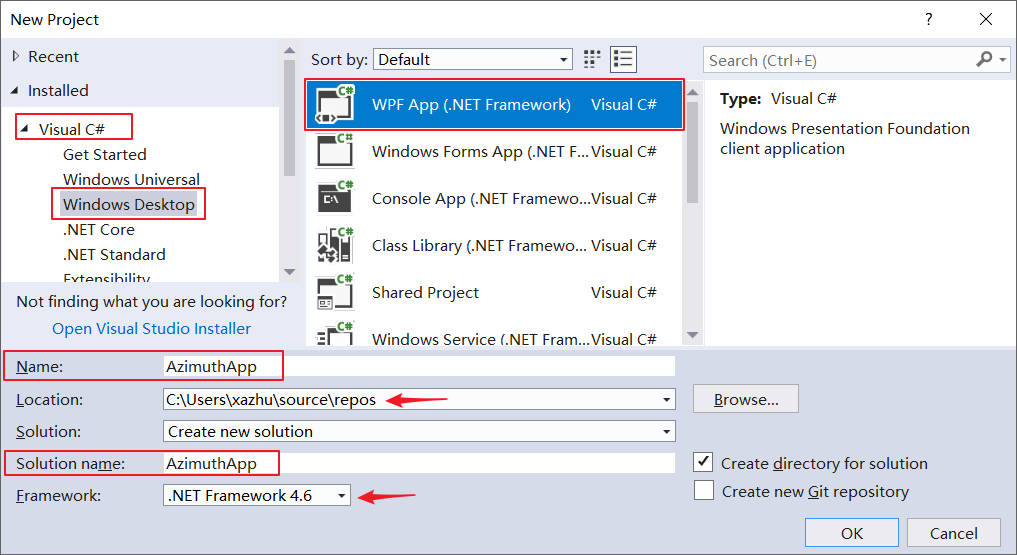
\includegraphics[scale=0.6]{surveybase/AzimuthApp1.png}
	\caption{新建项目示意图}
	\label{fig:AzimuthApp1}
\end{figure}

建好后的项目如图\ref{fig:AzimuthApp2}所示:

\begin{figure}[htbp]
	\centering
	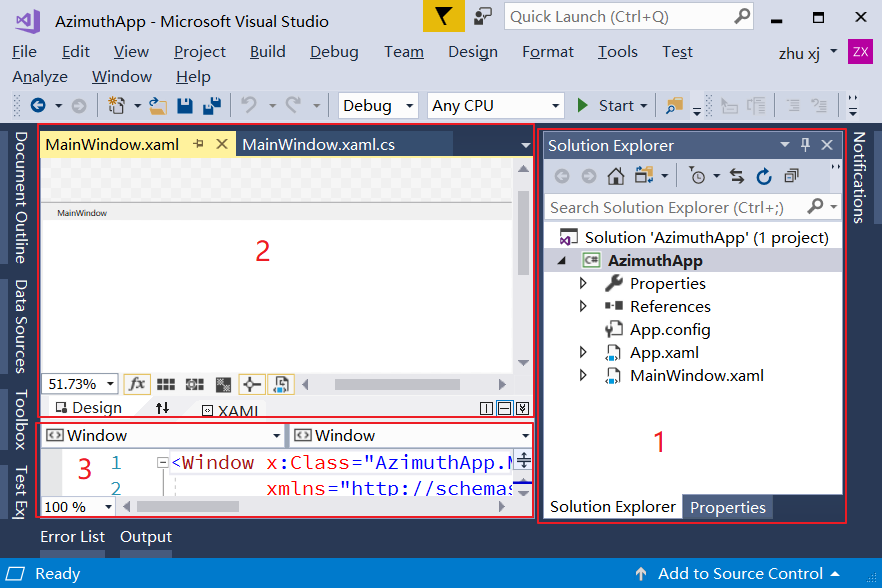
\includegraphics[scale=0.6]{surveybase/AzimuthApp2.png}
	\caption{方位角计算项目示意图}
	\label{fig:AzimuthApp2}
\end{figure}

由图\ref{fig:AzimuthApp2}可以看出,Visual Studio是以Solution、Project、File
的形式组织管理的。一个Solution可以包括一个至多个Project,一个Project中包含多个文件,
且一个Project编译为一个exe或dll文件,C\#中所有的对象与数据均以文件的形式组织。

图\ref{fig:AzimuthApp2}中的1区为Solution Explorer区,可对Project及File进行各种
操作。2、3区为代码与界面编写区,文件类型不同,呈现的内容也会不一样。

现代软件开发应遵循界面与算法分离的原则,因此我们再新建一类库项目SMath,用于
组织我们的算法,如图\ref{fig:AzimuthApp3}所示:

\begin{figure}[htbp]
	\centering
	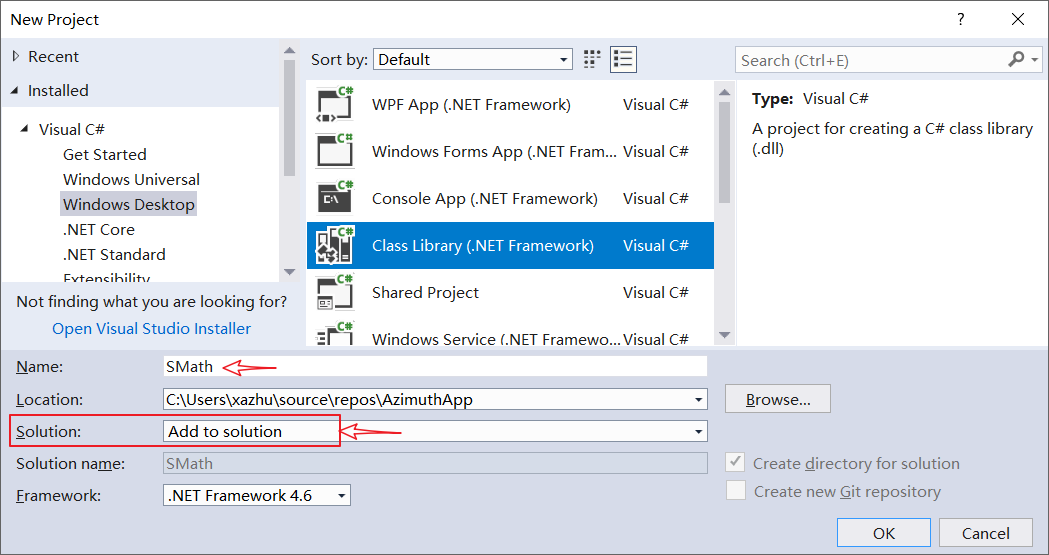
\includegraphics[scale=0.6]{surveybase/AzimuthApp3.png}
	\caption{新建类库项目示意图}
	\label{fig:AzimuthApp3}
\end{figure}

在该步操作中除了项目类型应选择Class Library之外,与图\ref{fig:AzimuthApp1}
不同的是此处Solution项应选择Add to solution而不是原来的 Create new solution。

现代软件开发的另一个原则是保证代码的可测试性,在增加类库项目后,
再增加一单元测试项目UnitTestSMath。鼠标右击图\ref{fig:AzimuthApp2}中的Solution Explorer区
中的Solution 'AzimuthApp'项,在弹出的右键快捷菜单中选择 Add,
在 Add 的下级菜单中选择 New Project..., 将弹出如图\ref{fig:AzimuthApp6}所示的添加单元测试项目的
对话框。

\begin{figure}[htbp]
	\centering
	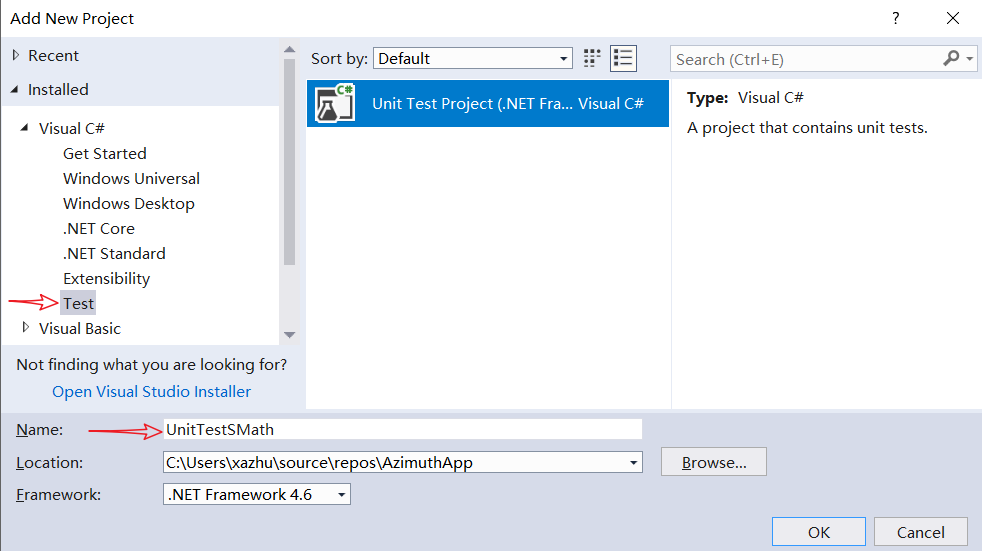
\includegraphics[scale=0.6]{surveybase/AzimuthApp6.png}
	\caption{添加单元测试项目示意图}
	\label{fig:AzimuthApp6}
\end{figure}

在图\ref{fig:AzimuthApp6}的操作中,应在左侧选择Test,在右边选择 Unit Test Project,

整个操作完成后,我们的解决方案Solution就拥有三个项目了,如图\ref{fig:AzimuthApp7}所示。
项目AzimuthApp为我们的界面编写项目,是启动项目(StartUp Project)。
项目SMath为我们的算法项目,项目UnitTestSMath为
对算法项目SMath进行单元测试的项目。

\begin{figure}[htbp]
	\centering
	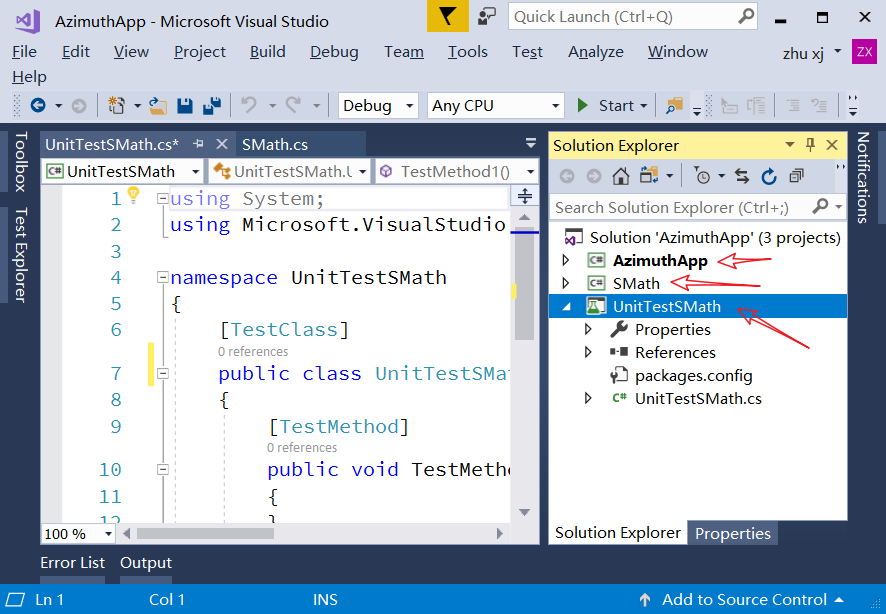
\includegraphics[scale=0.7]{surveybase/AzimuthApp7.png}
	\caption{完整的Solution示意图}
	\label{fig:AzimuthApp7}
\end{figure}

下面我们通过添加引用或参考(Add Reference)为三个项目建立关系。

SMath项目为基础算法,AzimuthApp需要用到其中的算法,因此应该向AzimuthApp项目
添加对SMath项目的引用。点击AzimuthApp项目将其展开,鼠标右击项目中的References
项,弹出如图\ref{fig:AzimuthApp4}所示的快捷菜单:

\begin{figure}[htbp]
	\centering
	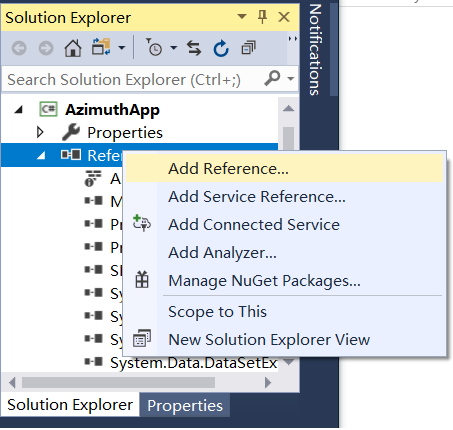
\includegraphics[scale=0.8]{surveybase/AzimuthApp4.png}
	\caption{引用类库项目示意图}
	\label{fig:AzimuthApp4}
\end{figure}

点击Add Reference...项,弹出如图\ref{fig:AzimuthApp5}所示的对话框。
在对话框左侧确保选中Projects,在右侧选中SMath项目,单击OK按钮就将引用添加完毕。
同样的方法向UnitTestSMath项目添加对SMath项目的引用。
\begin{figure}[htbp]
	\centering
	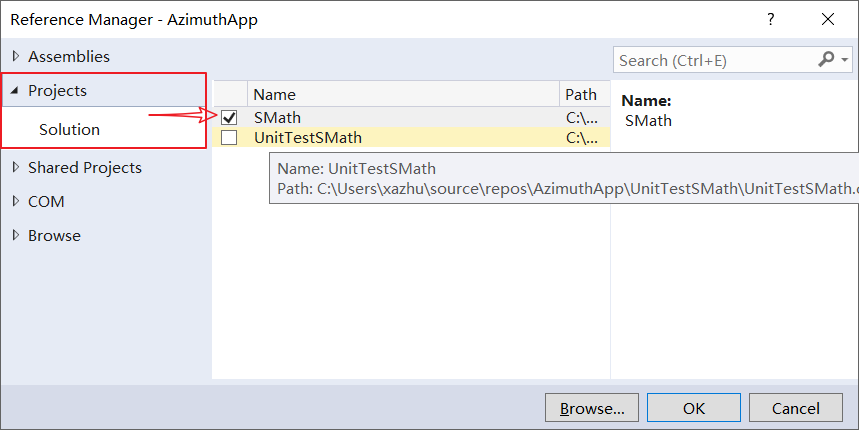
\includegraphics[scale=0.7]{surveybase/AzimuthApp5.png}
	\caption{选择引用类库项目示意图}
	\label{fig:AzimuthApp5}
\end{figure}

至此,我们的项目构建完成,整个程序的架构已经搭建好了。
在SMath项目中将原来的Class1.cs文件删除,新添一SMath.cs
文件,在SMath.cs文件中将我们前边讲解的SMath类加入其中,将各个函数组织进来,
对该项目执行构建(build)操作生成Dll类库文件,在另两个项目中就可以使用了。

\subsection{对算法进行单元测试}

SMath项目中的各个函数是我们的基础测量算法函数,必须保证它们的正确性。
为此对其编写单元测试函数进行严格的测试。如果以后需要对这些算法进行优化,
执行这些单元测试函数也可确保优化后的算法正确性。

点击展开UnitTestSMath项目,鼠标右键点击原来的文件UnitTest1.cs,
在弹出的菜单中选择Rename命令,将其改名为UnitTestSMath.cs,
在弹出的确认对话框中选择按钮 `是(Y)'就可以将其中的类名改为UnitTestSMath了。

我们首先编写DMStoDMS函数的测试函数,其代码如下:

\begin{lstlisting}[language=C]
//UnitTestSMath.cs文件内容
using System;
using Microsoft.VisualStudio.TestTools.UnitTesting;

namespace UnitTestSMath
{
    [TestClass]
    public class UnitTestSMath
    {
        [TestMethod]
        public void TestDMStoDMS()
        {
            ZXY.SMath.DMStoDMS(1.4, out int d, out int m, out double s);
            Assert.AreEqual(1, d);
            Assert.AreEqual(40, m);
            Assert.AreEqual(0, s, 1e-8);

            ZXY.SMath.DMStoDMS(-1.4, out d, out m, out s);
            Assert.AreEqual(-1, d);
            Assert.AreEqual(-40, m);
            Assert.AreEqual(0, s, 1e-8);

            ZXY.SMath.DMStoDMS(235.07492345, out d, out m, out s);
            Assert.AreEqual(235, d);
            Assert.AreEqual(7, m);
            Assert.AreEqual(49.2345, s, 1e-8);

            ZXY.SMath.DMStoDMS(-235.07492345, out d, out m, out s);
            Assert.AreEqual(-235, d);
            Assert.AreEqual(-7, m);
            Assert.AreEqual(-49.2345, s, 1e-8);
        }
    }
}
\end{lstlisting}

测试的原理非常简单,那就是已知一个值,让它经过一系列的运算得到期望的值。如果算法结果
与期望值相符,则测试通过,否则测试就不通过。

在Visual Studio系统中,单元测试的主要函数在Assert类中,其静态重载函数AreEqual
用于判断期望值(expected)与实际运算值(actual)是否相等。对于上述代码中d与m,由于
是整数,可以直接判断是否相等,而s是double类型,需给出一定的容错范围,不能直接判断
是否相等。

在测试代码中,我们分别用$1^{\degree} 40'$、$-1^{\degree} 40'$、
$235^{\degree} 07'49.2345''$、$-235^{\degree} 07'49.2345''$进行
测试,确保秒后第8位小数的准确性。

依次点击菜单栏上的Test -> Run -> All Tests 菜单项,在左侧的侧栏Test Explorer中
就可以显示测试结果,如图\ref{fig:AzimuthApp8}所示,图中左侧Test Explorer中测试项
显示为绿色,表明测试通过。

\begin{figure}[htbp]
    \centering
    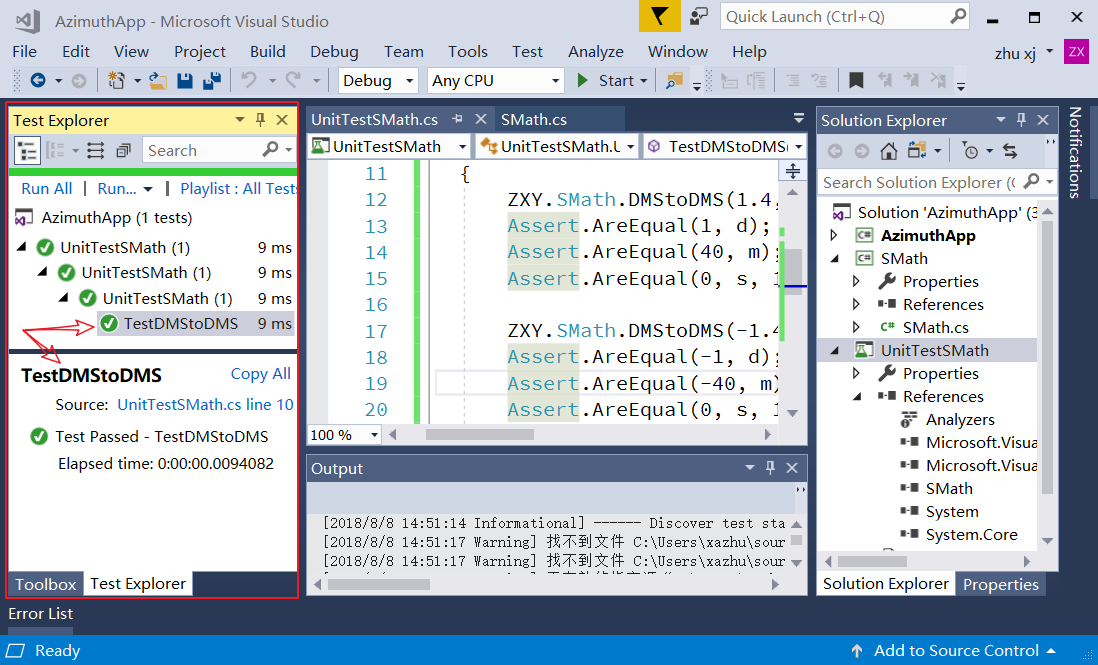
\includegraphics[scale=0.65]{surveybase/AzimuthApp8.png}
    \caption{执行单元测试成功的示意图}
    \label{fig:AzimuthApp8}
\end{figure}

如果我们将第30行代码中的-7改为-8,再执行测试命令,执行结果如图\ref{fig:AzimuthApp9},
图中左侧Test Explorer中测试项显示为红色的``×'',表明相应测试项未通过。

在Test Explorer下部显示了未通过测试的函数名称,位于源代码的哪一行,期望值是-8,
而实际值为-7。我们就可以根据这些信息去修正未通过测试的函数。

\begin{figure}[htbp]
    \centering
    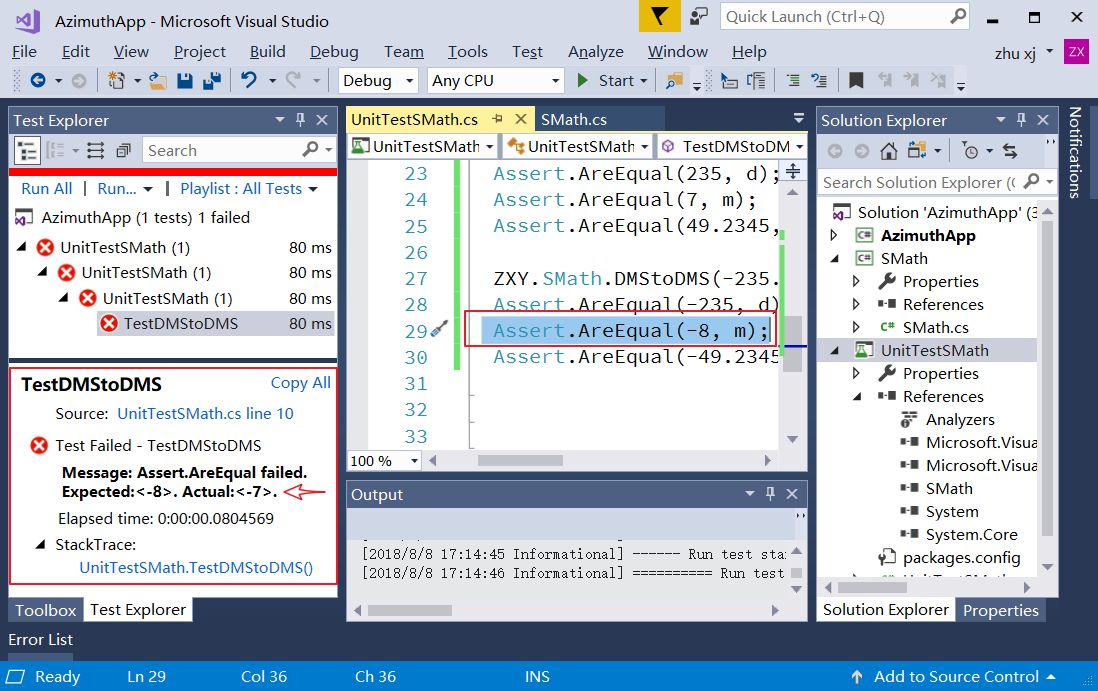
\includegraphics[scale=0.65]{surveybase/AzimuthApp9.png}
    \caption{执行单元测试失败的示意图}
    \label{fig:AzimuthApp9}
\end{figure}

由图\ref{fig:AzimuthApp8}与图\ref{fig:AzimuthApp9}可看出,测试通过,相应函数测试项
显示为绿色,测试项中之一不能通过,则相应函数测试项显示为红色。这就免去了我们人工再去比对的
环节,也利于机器的自动测试实施。

\subsection{界面编写}

在确保基本算法的正确性后,我们就可以编写界面程序了。我们编写一简单界面,如图\ref{fig:AzimuthUI1}
所示。

\begin{figure}[htbp]
    \centering
    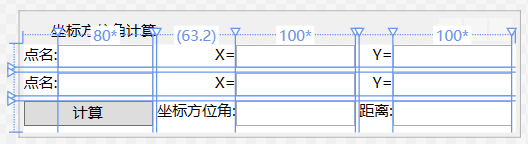
\includegraphics[scale=1]{surveybase/AzimuthUI1.png}
    \caption{坐标方位角计算设计界面}
    \label{fig:AzimuthUI1}
\end{figure}

相应的XAML设计代码如下:

\begin{lstlisting}[language=C]
<Window x:Class="AzimuthApp.MainWindow"
        xmlns="http://schemas.microsoft.com/winfx/2006/xaml/presentation"
        xmlns:x="http://schemas.microsoft.com/winfx/2006/xaml"
        xmlns:d="http://schemas.microsoft.com/expression/blend/2008"
        xmlns:mc="http://schemas.openxmlformats.org/markup-compatibility/2006"
        xmlns:local="clr-namespace:AzimuthApp"
        mc:Ignorable="d"
        Title="坐标方位角计算" Height="100" Width="400">
    <Grid>
        <Grid.ColumnDefinitions>
            <ColumnDefinition Width="Auto"/>
            <ColumnDefinition Width="80*"/>
            <ColumnDefinition Width="3"/>
            <ColumnDefinition Width="Auto"/>
            <ColumnDefinition Width="100*"/>
            <ColumnDefinition Width="3"/>
            <ColumnDefinition Width="Auto"/>
            <ColumnDefinition Width="100*"/>
            <ColumnDefinition Width="3"/>
        </Grid.ColumnDefinitions>
        <Grid.RowDefinitions>
            <RowDefinition Height="Auto"/>
            <RowDefinition Height="3"/>
            <RowDefinition Height="Auto"/>
            <RowDefinition Height="3"/>
            <RowDefinition Height="Auto"/>
        </Grid.RowDefinitions>
        <TextBlock Text="点名:" Grid.Row="0" Grid.Column="0" />
        <TextBox x:Name="textBoxAName" Grid.Row="0" Grid.Column="1" />
        <TextBlock Text="X=" TextAlignment="Right" Grid.Row="0" Grid.Column="3"/>
        <TextBox x:Name="textBoxAX" Grid.Row="0" Grid.Column="4"/>
        <TextBlock Text="Y=" TextAlignment="Right" Grid.Row="0" Grid.Column="6"/>
        <TextBox x:Name="textBoxAY" Grid.Row="0" Grid.Column="7" />

        <TextBlock Text="点名:" Grid.Row="2" Grid.Column="0" />
        <TextBox x:Name="textBoxBName" Grid.Row="2" Grid.Column="1" />
        <TextBlock Text="X=" TextAlignment="Right" Grid.Row="2" Grid.Column="3"/>
        <TextBox x:Name="textBoxBX" Grid.Row="2" Grid.Column="4" />
        <TextBlock Text="Y=" TextAlignment="Right" Grid.Row="2" Grid.Column="6"/>
        <TextBox x:Name="textBoxBY" Grid.Row="2" Grid.Column="7" />

        <Button x:Name="buttonAzimuth" Content="计算" Grid.Row="5" 
            Grid.Column="0" Grid.ColumnSpan="2" Click="buttonAzimuth_Click"/>
        <TextBlock x:Name="textBlockAzimuth" 
            Text="坐标方位角:" TextAlignment="Right" Grid.Row="5" Grid.Column="3"/>
        <TextBox x:Name="textBoxAzimuth" Grid.Row="5" Grid.Column="4" />
        <TextBlock Text="距离:" TextAlignment="Right" Grid.Row="5" Grid.Column="6" />
        <TextBox x:Name="textBoxDistance" Grid.Row="5" Grid.Column="7" />
    </Grid>
</Window>
\end{lstlisting}

计算按钮的Click事件代码如下:
\begin{lstlisting}[language=C]
private void buttonAzimuth_Click(object sender, RoutedEventArgs e)
{
    double.TryParse(textBoxAX.Text, out double xA);
    double.TryParse(textBoxAY.Text, out double yA);
    double.TryParse(textBoxBX.Text, out double xB);
    double.TryParse(textBoxBY.Text, out double yB);

    double distanceAB = ZXY.SMath.Azimuth(xA, yA, xB, yB, out double azimuthAB);

    textBoxAzimuth.Text = ZXY.SMath.RADtoString(azimuthAB);
    textBoxDistance.Text = distanceAB.ToString();
    textBlockAzimuth.Text = $"{textBoxAName.Text}->{textBoxBName.Text}坐标方位角:";
}
\end{lstlisting}

程序的运行结果如图\ref{fig:AzimuthUI2}所示。

\begin{figure}[htbp]
    \centering
    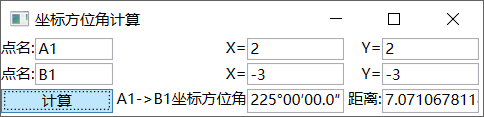
\includegraphics[scale=1]{surveybase/AzimuthUI2.png}
    \caption{坐标方位角计算运行界面}
    \label{fig:AzimuthUI2}
\end{figure}

\subsection{界面程序的优化}

WPF技术的核心是绑定(Binding),以上程序虽然简单,但也涉及数据与界面的交互问题。
我们对其界面稍加抽象,改写一下。

我们新建一个类AzimuthUI,其代码如下:
\begin{lstlisting}[language=C]
using System.ComponentModel;

namespace AzimuthApp
{
    class AzimuthUI : INotifyPropertyChanged
    {
        public event PropertyChangedEventHandler PropertyChanged;
        public void RaisePropertyChanged(string propertyName)
        {
            if (PropertyChanged != null)
            {
                PropertyChanged.Invoke(this, new PropertyChangedEventArgs(propertyName));
            }
        }

        private string _AName = "";
        public string AName
        {
            get => _AName;
            set
            {
                _AName = value;
                RaisePropertyChanged("AName");
            }
        }

        private double _xA;
        public double XA
        {
            get => _xA;
            set
            {
                _xA = value;
                RaisePropertyChanged("XA");
            }
        }


        private double _yA;
        public double YA
        {
            get => _yA;
            set
            {
                _yA = value;
                RaisePropertyChanged("YA");
            }
        }

        private string _BName = "";
        public string BName
        {
            get => _BName;
            set
            {
                _BName = value;
                RaisePropertyChanged("BName");
            }
        }

        private double _xB;
        public double XB
        {
            get => _xB;
            set
            {
                _xB = value;
                RaisePropertyChanged("XB");
            }
        }

        private double _yB;
        public double YB
        {
            get => _yB;
            set
            {
                _yB = value;
                RaisePropertyChanged("YB");
            }
        }

        public string AzimuthName
        {
            get => $"{AName}->{BName}坐标方位角:";
        }

        private double _azimuthAB;
        public string AzimuthAB
        {
            get => ZXY.SMath.RADtoString(_azimuthAB);
        }

        private double _distanceAB;
        public double DistanceAB
        {
            get => _distanceAB;
        }

        public void CalAzimuthDistanceAB()
        {
            _distanceAB = ZXY.SMath.Azimuth(XA, YA, XB, YB, out _azimuthAB);
            RaisePropertyChanged("AzimuthAB");
            RaisePropertyChanged("DistanceAB");
            RaisePropertyChanged("AzimuthName");
        }
    }
}
\end{lstlisting}

界面代码做如下修改:
\begin{lstlisting}[language=XML]
<TextBlock Text="点名:" Grid.Row="0" Grid.Column="0" />
    <TextBox x:Name="textBoxAName" Text="{Binding AName}" 
         Grid.Row="0" Grid.Column="1" />
    <TextBlock Text="X=" TextAlignment="Right"
         Grid.Row="0" Grid.Column="3"/>
    <TextBox x:Name="textBoxAX" Text="{Binding XA}" 
         Grid.Row="0" Grid.Column="4"/>
    <TextBlock Text="Y=" TextAlignment="Right" 
         Grid.Row="0" Grid.Column="6"/>
    <TextBox x:Name="textBoxAY" Text="{Binding YA}" 
         Grid.Row="0" Grid.Column="7" />

    <TextBlock Text="点名:" Grid.Row="2" Grid.Column="0" />
    <TextBox x:Name="textBoxBName" Text="{Binding BName}" 
         Grid.Row="2" Grid.Column="1" />
    <TextBlock Text="X=" TextAlignment="Right" Grid.Row="2" Grid.Column="3"/>
    <TextBox x:Name="textBoxBX" Text="{Binding XB}" 
         Grid.Row="2" Grid.Column="4" />
    <TextBlock Text="Y=" TextAlignment="Right" Grid.Row="2" Grid.Column="6"/>
    <TextBox x:Name="textBoxBY"  Text="{Binding YB}" 
         Grid.Row="2" Grid.Column="7" />

    <Button x:Name="buttonAzimuth" Content="计算" Grid.Row="5" 
        Grid.Column="0" Grid.ColumnSpan="2"
        Click="buttonAzimuth_Click"/>
    <TextBlock x:Name="textBlockAzimuth" 
        Text="{Binding AzimuthName, Mode=OneWay}" 
        TextAlignment="Right" Grid.Row="5" Grid.Column="3"/>
    <TextBox x:Name="textBoxAzimuth" Text="{Binding AzimuthAB, Mode=OneWay}" 
        Grid.Row="5" Grid.Column="4" />
    <TextBlock Text="距离:" TextAlignment="Right" Grid.Row="5" Grid.Column="6" />
    <TextBox x:Name="textBoxDistance" Text="{Binding DistanceAB, Mode=OneWay}"
        Grid.Row="5" Grid.Column="7" />
\end{lstlisting}

MainWindow窗体的后代代码做如下修改:

\begin{lstlisting}[language=C]
namespace AzimuthApp
{
    public partial class MainWindow : Window
    {
        AzimuthUI azimuthUI;
        public MainWindow()
        {
            InitializeComponent();

            azimuthUI = new AzimuthUI();
            this.DataContext = azimuthUI;
        }

        private void buttonAzimuth_Click(object sender, RoutedEventArgs e)
        {
            azimuthUI.CalAzimuthDistanceAB();
        }
    }
}
\end{lstlisting}


\section*{作业}

\begin{enumerate}
\item 以上DMStoString函数与RADtoString函数可以正确的将角度值中的度分秒值提取出来并
以更好阅读的字符串$23\degree 05'47.6324''$形式表达。但对于负的角度会表达为
$-23\degree -05'-47.6324''$形式,对于追求完美的某些程序员来讲这似乎有些不可接受,
他们仍然想将负的角度表达为$-23\degree 05'47.6324''$或$-0\degree 05'47.6324''$
形式。请试着改进以上的DMStoString与RADtoString函数。
    
\item 请用Math.Atan函数编写两点坐标反算坐标方位角的函数Azimuth。

\item 请将单元测试项目UnitTestSMath中的测试函数TestAzimuth与TestRADtoDMS等补充
编写完整。
\end{enumerate}